\documentclass{article}
\usepackage[a4paper, margin=1in]{geometry}

\usepackage{graphicx}
\title{\vspace{-0.5in}\textbf{Simple 16-Bit CPU}}
\author{Sai Sudhir Sunku -- PES2UG21CS460 \\ Samarth Ramesh -- PES2UG21CS465 \\ Sanket Padhi -- PES2UG21CS477}
\date{}
\begin{document}
\maketitle
\section{Abstract}
Our project proposes and implements a 16-bit CPU, using a Harvard Architecture.
It has 16 bits of address-space, 16-bit words, and 18-bit wide instructions.

The CPU has been designed to be Stack based, as a result of which most of the memory operations are performed at the top. 
However, random access is also possible.

Two general purpose registers ``T'' and ``R'' have been provided for.
The ``T'' register is used as the first input for the ALU, the top of the stack being the second,  while the ``R'' is the output of the ALU.

The Stack Pointer (SP) is stored in the eponymous register.
The address of the instruction being executed is stored in the IP register.

The ALU itself is a COTS component, the venerable 74181 ALU, which supports 32 different operations.

The Instruction set supports 3 primary classes of instruction, data (``DT''), move (``MV'') and operate (``OP'').

\section{Schematic Diagram}
\begin{figure}[h!]
    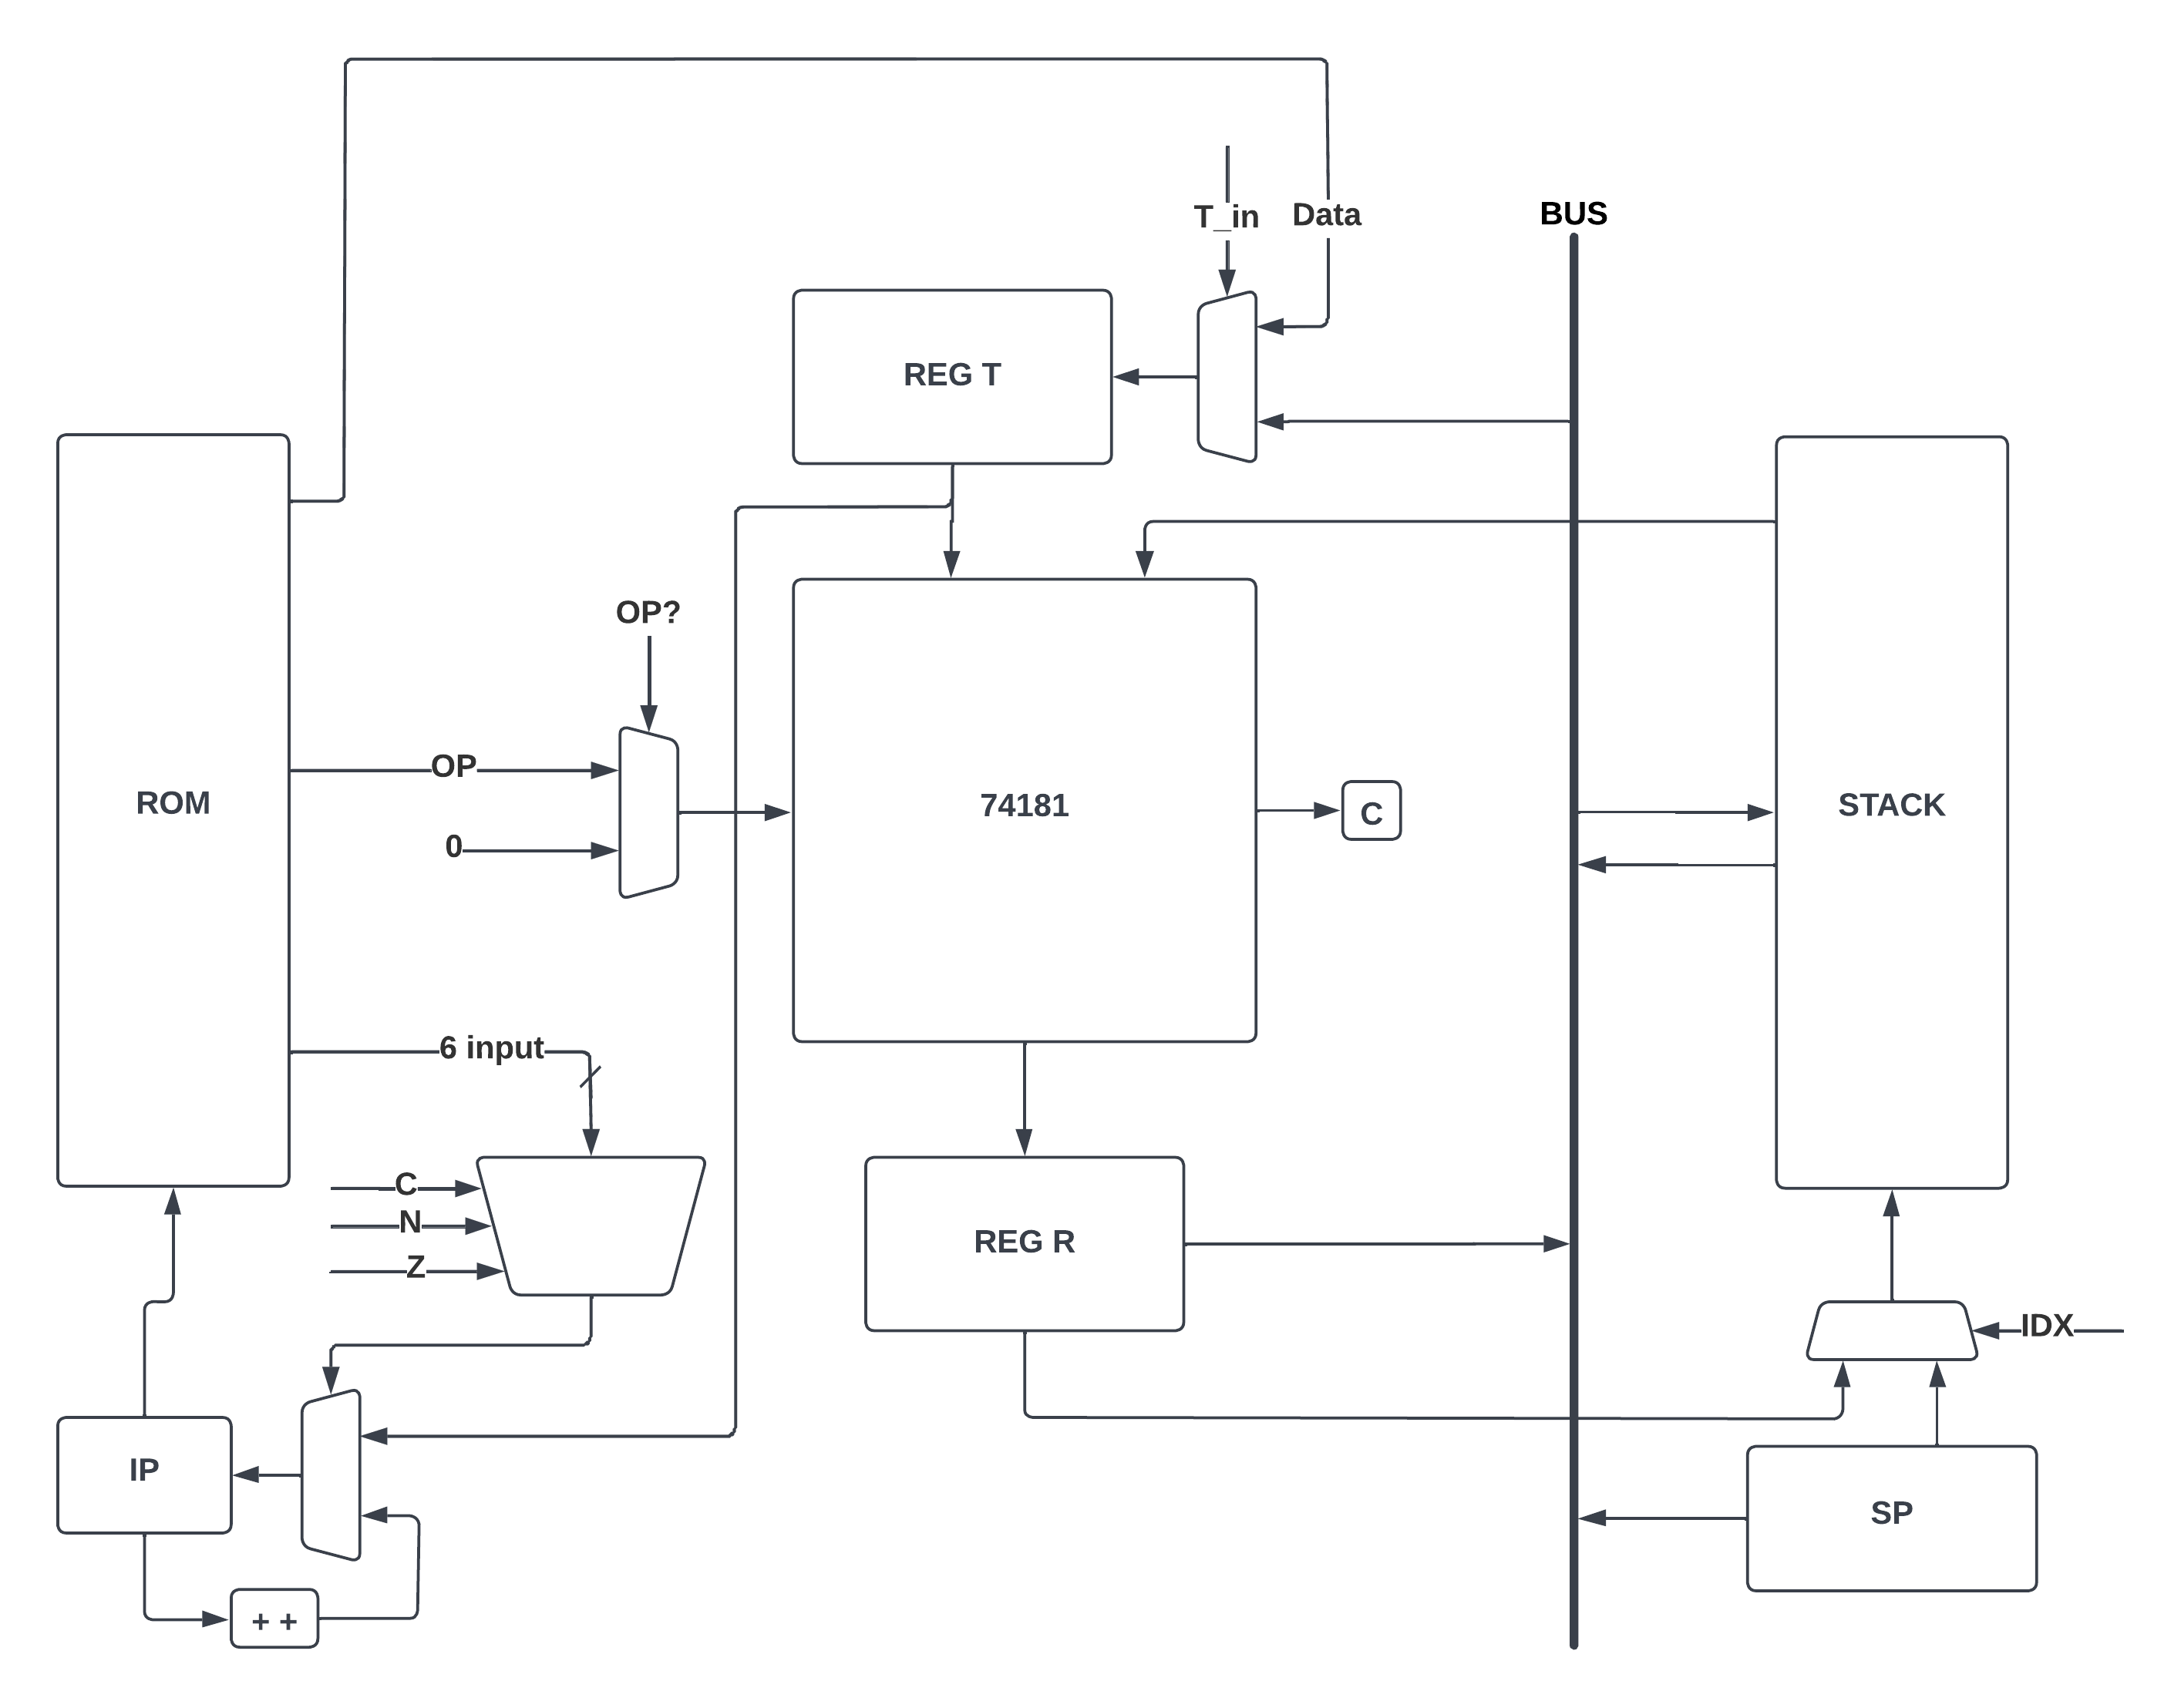
\includegraphics[scale=0.15]{cd.png}
    \centering
\end{figure}
\end{document}

